\documentclass{beamer}
\setbeameroption{show notes on second screen=right}

\usepackage{esint}
\usepackage{graphicx}
\usepackage{caption}
\usepackage[british]{babel}
%\usepackage{kpfonts}

% Theme (Boadilla, Hannover, metropolis, Pittsburgh)

% METROPOLIS
% Uses Fira fonts - compile with xelatex to use
% Features [standout] frames

\usetheme[progressbar=frametitle]{metropolis}

% Colours (owl, dolphin, seagull)

% OWL
% Custom colours: red, green, blue, cyan, brown, orange, yellow, violet
% Has [snowy] variant

\usecolortheme{}

\useinnertheme{}                            % Bullet point style (circles usually best)
\useoutertheme{}                       % Header/footer style
\setbeamerfont{caption}{size=\tiny}         % Caption size
\captionsetup[figure]{labelformat=empty}    % Remove figure labels
\usefonttheme[onlymath]{serif}

%\logo{\includegraphics[height=2cm]{}}
\title{Music Arrangement via Quantum Annealing}
\subtitle{}
\author{Lucas Kirby}
\institute{\color{violet} Durham University}
\date{\today}

\begin{document}

\begin{frame}
    \titlepage
\end{frame}

\begin{frame}{Overview}
    \tableofcontents
\end{frame}

% Example centered frame
\begin{frame}[standout]
    \centering
    What is flux?
\end{frame}

\section{Theory}
\subsection{Arrangement}
\subsection{Quantum annealing}

\begin{frame}{Column layout}
    \begin{columns} % Two column layout

        \begin{column}{0.6\textwidth} % Left column slightly bigger
            \begin{itemize} % Bullet points (\enumerate for numbers)
                % Reveal bullet points at a time
                \item<2-> \color{red} Net flux of liquid is zero
                \item<3-> \color{blue} Sources provide net outwards flow
                \item<4-> \color{green} Sinks provide net inwards flow
            \end{itemize}
        \end{column}

        \begin{column}{0.4\textwidth}
            \begin{figure}
                \centering
                    \includegraphics<1->[width=\textwidth]{../Figures/problemGraph.pdf} % Reveal order after \command
                    \caption{\color{orange} Source: Wikimedia Commons}
                \end{figure}
        \end{column}

    \end{columns}
\end{frame}

\section{Methods}
\section{Results}

\begin{frame}{Blocks}
    \begin{equation*}
        \oiint_A E\cdot dA=\frac{Q}{\varepsilon_0}
    \end{equation*}
    \pause
    \begin{block}{} % Empty title
        \centering
        The \emph{net electric flux} through any \alert{closed} surface is proportional to the \textbf{enclosed charge}.
    \end{block}

    \begin{alertblock}{Alert}
        This is an alert.
    \end{alertblock}

    \begin{exampleblock}{Example}
        This is an example.
    \end{exampleblock}
        
\end{frame}

\begin{frame}{Equation alignment}
    \begin{align*} % Aligning on [=]
        \onslide<1-5>{F&=-\frac{GMm}{r^2}} \\
        \onslide<2-5>{g&=-\frac{GM}{r^2}} \\
        \onslide<3-5>{g\cdot 4\pi r^2&=-4\pi GM} \\
        \onslide<4-5>{g \oiint_A dA&=-4\pi GM}\\
        \onslide<5->{\oiint_A g\cdot dA&=-4\pi GM}
    \end{align*}

    \begin{block}{}<6-> 
        \centering
        The gravitational flux through any closed surface is proportional to the enclosed mass.
    \end{block}
\end{frame}

\begin{frame}{Apperance sync}
    \begin{columns}

        \begin{column}{0.6\textwidth}
            \begin{itemize}
                \item<2-> Volume rate of flow equal to divergence
                \item<3-> Summed over entire volume
                \item<4-> Equal to net flow across the boundary
            \end{itemize}
        \end{column}

        \begin{column}{0.4\textwidth}
            \begin{figure}
                \centering
                    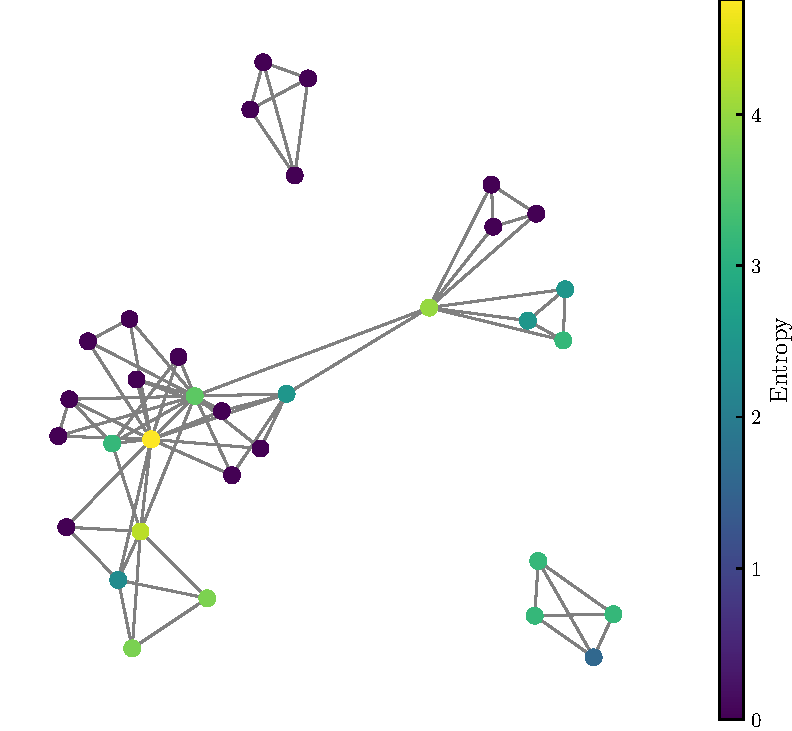
\includegraphics[width=\textwidth]{../Figures/problemGraph.pdf}
                    \caption{Source: Wikimedia Commons}
            \end{figure}
            \begin{equation*}
                % Syncing equation appearance with bullet points
                \onslide<3->{\iiint_V}\onslide<2->{\nabla\cdot\textbf{F}}\onslide<3->{\,dV}\onslide<4->{=\oiint_A \textbf{F}\cdot d\textbf{A}}
            \end{equation*}
        \end{column}

    \end{columns}
\end{frame}

\section{Conclusions}

\begin{frame}{Equation gather}
    \begin{gather*} % Multiple equations if alignment not important
        \nabla\cdot \textbf{E}=\frac{\rho}{\varepsilon_0} \\
        \nabla\cdot \textbf{B}=0 \\
        \nabla\times \textbf{E}=-\frac{\partial \textbf{B}}{\partial t} \\
        \nabla\times \textbf{B}=\frac1{c^2}\frac{\partial \textbf{E}}{\partial t}+\mu_0I
    \end{gather*}
\end{frame}

\end{document}